\documentclass[aspectratio=169,t,11pt,table]{beamer}
\usepackage{../../slides,../../math}

% Optionally define `accent`/`accent2` colors for theme customization
% I recommend changing the top slider on this: https://hslpicker.com/#1e9400
\definecolor{accent}{HTML}{2B5269}
\definecolor{accent2}{HTML}{9D2235}

\title{Topic 1: Introduction to Causal Inference and Potential Outcomes Framework}
\subtitle{\it  ECON 5783 — University of Arkansas}
\date{Fall 2025}
\author{Prof. Kyle Butts}

\begin{document}

% ------------------------------------------------------------------------------
\begin{frame}[noframenumbering,plain]
  \maketitle

  % \bottomleft{\footnotesize $^*$A bit of extra info here. Add an asterich to title or author}
\end{frame}
% ------------------------------------------------------------------------------

\begin{frame}{Potential Outcomes Framework}
  We learn:
  \begin{itemize}
    \item How to think of Causal Effects in terms of "All Else Equal"
    \item What are ``Potential Outcomes''?
    \item Identifying causal effects via randomized experiments
  \end{itemize}

  \bigskip
  Readings to complement this lecture are:
  \begin{itemize}
    \item Cunningham (2021) \emph{Causal Inference: The Mixtape}, Chapters 4
    
    \item Good summary videos: \url{https://www.youtube.com/watch?v=lFKYfCeXiI4} and \url{https://www.youtube.com/watch?v=jVkQPnARPQ0}
  \end{itemize}
\end{frame}

\begin{frame}{Causal Inference}
  The goal of the class is to think about establishing \emph{causal} relationships:
  \begin{itemize}
    \item Given some outcome, $Y$, that we care about, we want to know if changing $X$ \emph{causes} a change in $Y$
  \end{itemize}
    
  \pause
  \bigskip
  In the real world, we can only observe whether $X$ and $Y$ co-move (\alert{statistical inference}) but trying to know if $X$ caused $Y$ (\alert{causal inference}) is much more difficult a problem
  \begin{itemize}
    \item We will try to tackle this problem, but be humble of the difficulties of this task
  \end{itemize}
\end{frame}

\begin{frame}{The Enlightenment Era and The Scientific Method}
  In some sense, the methods of establish causal links date back to the Enlightenment Era
  \begin{itemize}
    \item Empiricism, Experimentation, and `Reasoning' led to many scientific breakthroughs and, some scholars argue, was essential for the Industrial Revolution (e.g. Joel Mokyr)
  \end{itemize}

  \pause
  \bigskip
  They would have ``Scientific Societies'' that were basically large dinner parties where they would dicuss how to learn about the world (`experimentation') 
\end{frame}

\begin{frame}{Royal (Scientific) Society of London}
  \begin{columns}[T]
    \begin{column}{.55\textwidth}\vspace*{-\bigskipamount}
      \begin{center}
        \includegraphics[width = \textwidth]{figures/royal_society.jpg}
        % Source: 
        % https://en.wikipedia.org/wiki/File:Royal_Society,_Crane_Court,_off_Fleet_Street,_London;_a_meet_Wellcome_L0013032.jpg
      \end{center}
    \end{column}
    \begin{column}{.45\textwidth}
      Most famously, was the Scientific Society of London
      \begin{itemize}
        \item Ben Franklin's key and kite was written in a letter to the Society
      \end{itemize}
    \end{column}
  \end{columns}
\end{frame}

\begin{frame}{Scientific Society of London}{`Nullius in verba'}
  \begin{quote}
    The Royal Society's motto 'Nullius in verba' was adopted in its First Charter in 1662. is taken to mean 'take nobody's word for it'. It is an expression of the determination of Fellows to withstand the domination of authority and to verify all statements by an appeal to facts determined by experiment.

    Source: https://royalsociety.org
  \end{quote}
\end{frame}

\begin{frame}{Randomized Controlled Trial}
  The first randomized controlled trial (RCT) was conducted by James Lind in 1753
  \begin{itemize}
    \item Randomly assigned 12 sailors into 6 groups to have different potential `treatments'
  \end{itemize}

  \bigskip
  Citrus ended up winning out
\end{frame}

\begin{frame}{What makes an RCT work well?}
  In groups, let's think about what makes an RCT effective at identifying what the true effects of a treatment is

  \pause
  By \emph{randomly} giving people different treatments, we can be sure the groups are similar
  \begin{itemize}
    \item `Controlled' trial == making sure the units are comparable
  \end{itemize}
\end{frame}

\begin{frame}{``Observational'' version}
  Say, instead, that James Lind went out and surveyed a bunch of people
  \begin{itemize}
    \item Asked whether or not they had scurvy and whether or not they consumed citrus
  \end{itemize}
  
  \bigskip
  He documents that people that have a lot of citrus rarely have scurvy
  \begin{itemize}
    \item Why is this evidence much weaker? 
  \end{itemize}
\end{frame}

\begin{frame}{Random Allocation ensures comparability}
  \bigskip
  \begin{quote}
    Having used a random allocation, the sternest critic is unable to say when we eventually dash into print that quite probably the groups were differentially biased through our predilections or through our stupidity.

    \emph{—Austin Bradford Hill, 1952}
  \end{quote}
  % Quote taken from https://pmc.ncbi.nlm.nih.gov/articles/PMC8718586/#:~:text=The%20Opportunity%20and%20Challenges%20for%20Conducting%20RCTs,our%20stupidity.%20%E2%80%94Austin%20Bradford%20Hill%2C%201952%2010.
\end{frame}

\begin{frame}{The `Social Scientific Method'}
  What then are we to do when we try to establish causality in the messy messy world?

  \bigskip
  {\color{magenta} Option 1}: Run experiments. Get out in the world and run RCTs! 
  \begin{itemize}
    \item E.g. guaranteed income experiments, assigning a free lawyer for eviction court, micro-credit loans in developing countries
  \end{itemize}
\end{frame}

\begin{frame}{The `Social Scientific Method'}
  But, in many cases, we can not run experiments
  \begin{itemize}
    \item e.g. we care about the impacts of kids on parents, but can not randomly assign people to have kids
  \end{itemize}

  \bigskip
  {\color{magenta} Option 2}: Look for `natural experiments' in the world
  \begin{itemize}
    \item e.g. draft lottery; discrete cut-offs in policies; random cost shocks to firms
  \end{itemize}
\end{frame}

\begin{frame}{The `Social Scientific Method'}
  As our ability to approximate a random experiment worsens, the credibility of our estimates worsens as well
  \begin{itemize}
    \item The RCT is often called the `gold standard' for this reason
  \end{itemize}

  \bigskip
  {\color{magenta} Option 3}: Control for important variables and do as good as we can
\end{frame}

\begin{frame}{The `Social Scientific Method'}
  Sometimes we need to answer questions even if a natural experiment does not fall in our laps
  \begin{itemize}    
    \item But, this requries the \emph{most caution}; we will discuss strategies to approximate an experiment as best as we can
  \end{itemize}

  \bigskip
  \emph{Point of Caution:} Just because a question is important, does not mean we should throw away careful scientific rigor
\end{frame}

\begin{frame}{The Social Scientist' obligation}{A bit soap-boxy, but it's important}
  \begin{quote}
    The first principle is that you must not fool yourself — and you are the easiest person to fool.

    \emph{— Richard Feynman, 1974}
  \end{quote}

  \bigskip
  The key insight of the scientific method is to \emph{rule out potential alternative explanations}
  \begin{itemize}
    \item As much as possible, you want to \emph{prove your theory wrong}. 
  \end{itemize}

  \bigskip
  A good social scientist is an expert on the topic they are researching
  \begin{itemize}
    \item Just because you do not \emph{know} an alternative explanation, does not mean it does not exist
  \end{itemize}
\end{frame}


\begin{frame}{Social Scientific Method in Action}{The Enlightenment and the Industrial Revolution}
  In that spirit, let us go back to the original claim in this introduction: 
  ``scientific breakthroughs and, some scholars argue, was essential for the Industrial Revolution''

  \bigskip
  Is this true?
\end{frame}

\begin{frame}{Social Scientific Method in Action}{The Enlightenment and the Industrial Revolution}
    \begin{columns}[T]
    \begin{column}{.35\textwidth}\vspace*{-\bigskipamount}
      \begin{center}
        \includegraphics[width = 0.75\textwidth]{figures/encyclopedie.jpg}
      \end{center}
    \end{column}
    \begin{column}{.65\textwidth}
      Squicciarini and Voigtländer (2015, QJE) try to answer this using \emph{the Encylopedié}
      \begin{itemize}
        \item Published in France in 1751 and contained a bunch of evidence from Enlightenment scientists
      \end{itemize}

      \bigskip
      A single person in the town might buy this expensive book and share it with other people
    \end{column}
  \end{columns}
\end{frame}

\begin{frame}{Social Scientific Method in Action}{The Enlightenment and the Industrial Revolution}
  Squicciarini and Voigtländer (2015, QJE) digitized records of who purchased the Encyclopedié (7081 in total)
  \begin{itemize}
    \item In their sample of French cities, 85 had purchased one and 108 did not
  \end{itemize}
  
  \bigskip
  Comparing cities of similar size and geographic location, they find that cities with this scientific knowledge grew at faster rates than other cities
  \begin{itemize}
    \item With your groups, think about whether or not this is a good `experiment'  
  \end{itemize}
\end{frame}

\begin{frame}{Social Scientific Method in Action}{The Enlightenment and the Industrial Revolution}
  To bolster their evidence, they do:
  \begin{enumerate}
    \item Subscriber rate is uncorrelated with growth from 1400 to 1750 (potentially alleviating some concerns about which kinds of places subscribed)
    
    \item They include controls for port access, universities, and city density
  \end{enumerate}
\end{frame}

\begin{frame}{Social Scientific Method in Action}{Jon Snow and Cholera}
  Three major waves of cholera in the early to mid 1800s in London, largely thought to be spread by miasma (``dirty air'')
  \begin{itemize}
    \item No theory of the germ yet
  \end{itemize}
\end{frame}

\begin{frame}{Social Scientific Method in Action}{Jon Snow and Cholera}
  John Snow believed cholera was spread through the Thames water supply through an `invisible creature' that entered the body through food and drink
  
  \bigskip
  London passes ordinance requiring water utility companies to move inlet pipe further up the Thames, above the city center, but not everyone complies
  \begin{itemize}
    \item Natural experiment: Lambeth water company moves its pipe between 1849 and 1854; Southwark and Vauxhall water company delayed
  \end{itemize}

  \bigskip
  ``Staggered rollout'' of policies is a common empirical method
\end{frame}

\begin{frame}{Social Scientific Method in Action}{Computers and Wage Structure}
  Alan Krueger (1993, QJE) use a regression strategy and US survey data and documents that workers who use a computer earn 10-15\% more than those that do not
  \begin{itemize}
    \item Use a bunch of different regression methods and find `robust' results
  \end{itemize}

  \bigskip
  \pause
  DiNardo and Pischke (1997, QJE) revisit this analysis using German data
  \begin{itemize}
    \item Find similar estimates for computers
    
    \item But, find remarkably similar results for the use of pencils at work!!
  \end{itemize}

  \bigskip
  Don't forget to rule out potential explanations!
\end{frame}


% \begin{frame}{Research Strategy}
%   
% \end{frame}
% 
% https://economicspsychologypolicy.blogspot.com/2015/06/list-of-19-natural-experiments.html


\section{Difficulties of Establishing Causality}

\begin{frame}{Correlation does not imply Causality}
  \begin{columns}[T]
    \begin{column}{.6\textwidth}\vspace*{-\bigskipamount}
      \begin{center}
        \includegraphics[width = 0.75\textwidth]{figures/rooster_crowing_at_sun.jpg}
      \end{center}
    \end{column}
    \begin{column}{.4\textwidth}
      Rooster crowing does not cause sun to rise
      \begin{itemize}
        \item The rooster crows every morning when the sun comes up
      \end{itemize}
    \end{column}
  \end{columns}
\end{frame}

% \begin{frame}{Correlation does not imply causation}
%   \begin{columns}[T]
%     \begin{column}{.6\textwidth}\vspace*{-\bigskipamount}
%       \begin{center}
%         \includegraphics[width = 0.75\textwidth]{figures/sleeping_with_shoes.png}
%       \end{center}
%     \end{column}
%     \begin{column}{.4\textwidth}
%       Sleeping with one's shoes on is strongly correlated with waking up with a headache.
% 
%       \begin{itemize}
%         \item A common cause that leads to sleeping with shoes on and waking up with a headache
%       \end{itemize}
%     \end{column}
%   \end{columns}
% \end{frame}

\begin{frame}{Correlation does not imply causation}
  \begin{columns}[T]
    \begin{column}{.6\textwidth}\vspace*{-\bigskipamount}
      \begin{center}
        \includegraphics[width = 0.75\textwidth]{figures/wine_and_health.png}
      \end{center}
    \end{column}
    \begin{column}{.4\textwidth}
      Drinking wine is correlated with improved health

      \begin{itemize}
        \item Drinking wine is also correlated with income $\dots$
      \end{itemize}
    \end{column}
  \end{columns}
\end{frame}

\begin{frame}{Causality does not imply correlation}
  \begin{columns}[T]
    \begin{column}{.6\textwidth}\vspace*{-\bigskipamount}
      \begin{center}
        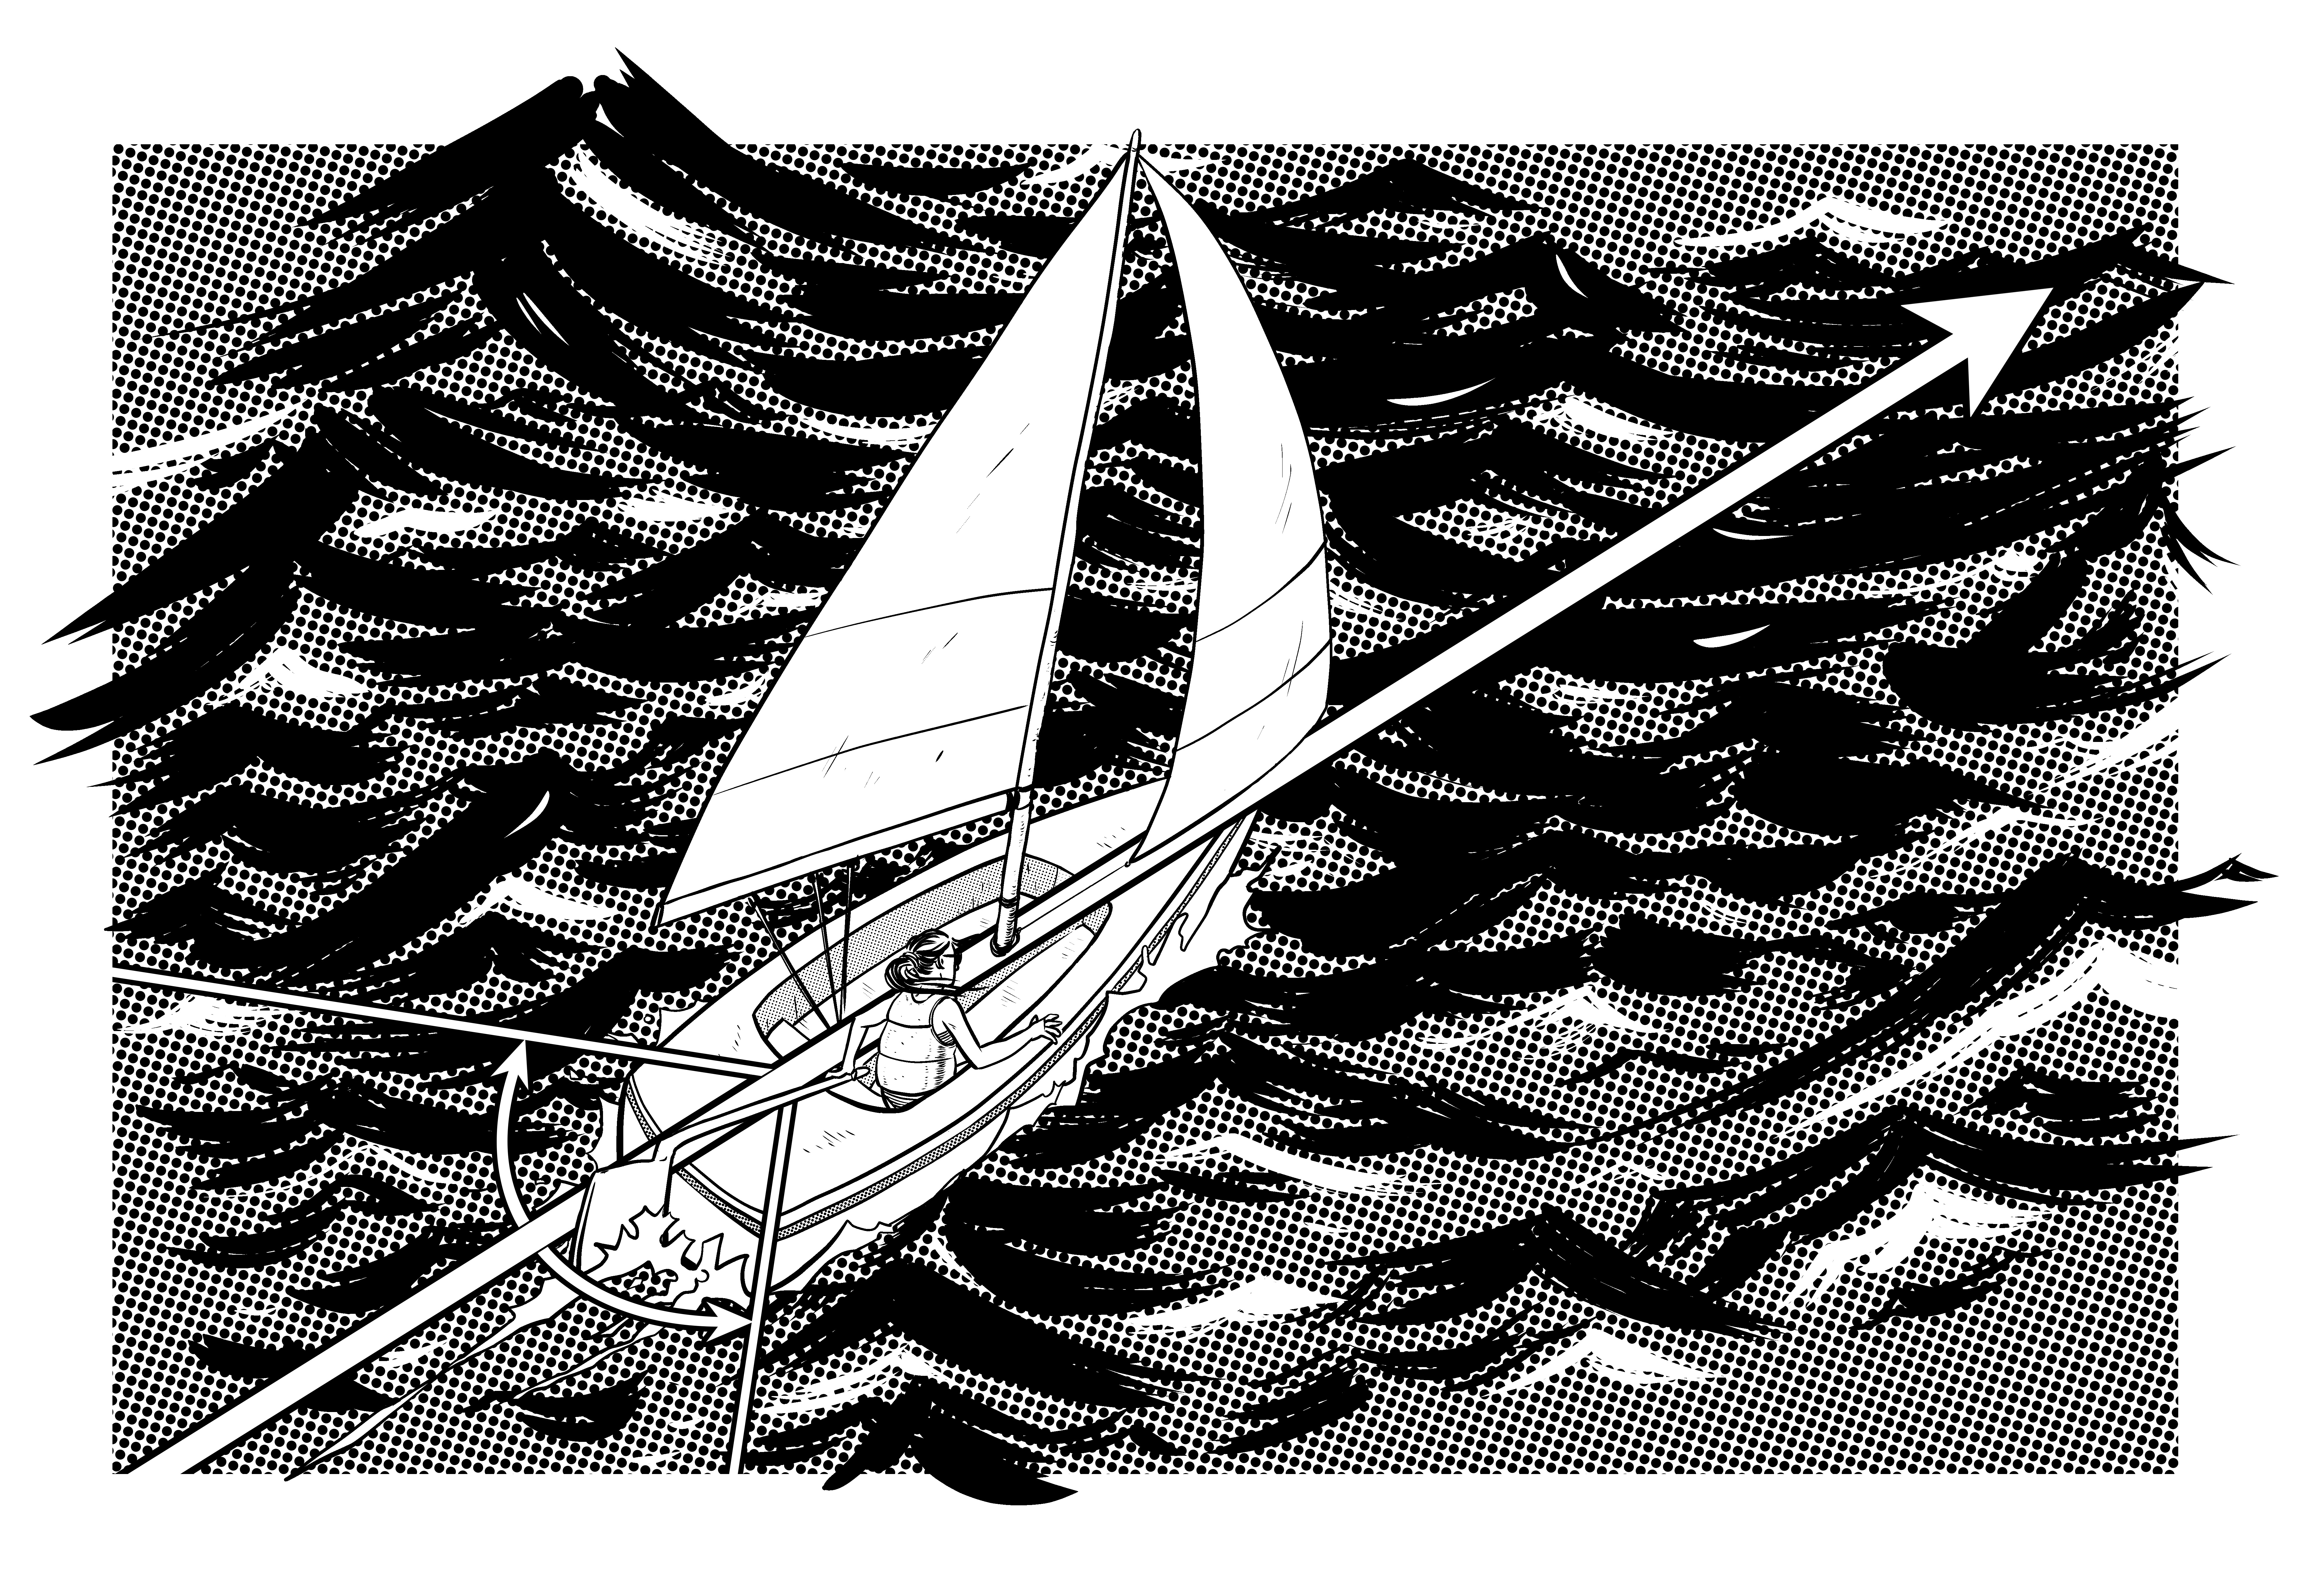
\includegraphics[width = \textwidth]{figures/scottboat.jpg}
      \end{center}
    \end{column}
    \begin{column}{.4\textwidth}
      A boat is traveling on a windy day
      \begin{itemize}
        \item The sailor turns the rudder back and forth
        \item Boat moves in a straight line
      \end{itemize}
      \bigskip
      No correlation between rudder direction and boat direction; but the rudder still \emph{causes} the boat to change direction
    \end{column}
  \end{columns}
\end{frame}

\begin{frame}{Causality does not imply correlation}
  \begin{columns}[T]
    \begin{column}{.6\textwidth}
			\vspace*{-\bigskipamount}
      \begin{center}
        \includegraphics[width = \textwidth]{figures/fed_balance_grey.jpg}
      \end{center}
    \end{column}
    \begin{column}{.4\textwidth}
      The federal reserve changes interest rates back and forth to try and keep inflation around target of 2\% 
      \begin{itemize}
        \item When things are going well, no correlation between interest rate and inflation rate
      \end{itemize}
    \end{column}
  \end{columns}
\end{frame}

\begin{frame}{Lurking variables}
  Correlations can often arise due to the presence of some third underlying variable that is driving both. We call this a \alert{lurking variable}
  \begin{itemize}
    \item Housing prices go up in places where they're building new apartments
    
    \item Employment goes up after places raise their minimum wage
    
    \item Schools with more arts spending have higher test scores
    
    \item Correlates of food consumption and health
    
    % \item Places with more police officers have more crime 
  \end{itemize}
\end{frame}

\begin{frame}{Lurking variables}
  In all of these examples, there seems to be other explanations \alert{lurking around the corner}:
  \begin{itemize}
    \item New apartments are built in neighborhoods with growing demand
    
    \item The minimum wage is passed in places with a growing economy
    
    \item Schools with more arts spending are in wealthier school districts
    
    \item Food consumption and health are both correlated with income
    
    % \item Places with more crime have more police officer
  \end{itemize}
\end{frame}

\begin{frame}{Reverse Causality}
  Sometimes we have the order of causation \emph{reversed}:
  \begin{itemize}
    \item People who drink more coffee have more anxiety
    
    \item Places with more police officers have more crime 
    
    \item People who try new medicines have higher mortality rates
  \end{itemize}
 f
  \bigskip
  We want to think carefully if $X$ causes $Y$ or $Y$ causes $X$
\end{frame}

\begin{frame}{The Encyclopedié}
  One main concern with Squicciarini and Voigtlände's approach is reverse causality
  \begin{itemize}
    \item Places with more innovations might seek out more scientific knowledge (growth causing subscriptions)
  \end{itemize}

  \bigskip
  To address this, they use the presence of historic scientific society to `predict' which places would buy an Encyclopedié
  \begin{itemize}
    \item This is called an `instrument' which we will discuss later in this class
  \end{itemize}
\end{frame}

\section{Counterfactual Thinking and Potential Outcomes}

\begin{frame}{What is causality?}
  The goal of \alert{causality} is to try and figure out how if I were to change some variable $X$ \emph{at some point in time}, how would the value of $Y$ change for that person
  \begin{itemize}
    \item We have some notion of `changing' $X$ in some `experimental' or `random' way
  \end{itemize}

  \pause
  \bigskip
  \alert{PROBLEM:} we can \emph{never} observe both states of the world \emph{at the same point in time}.
\end{frame}

\begin{frame}{Observational Studies}
  When we look out into the world, people have different $X$s. Why can we not just compare $Y$s for people with different values of $X$? 
  
  \begin{itemize}
    \item As economists, we know that people are optimizers. They chose their `optimal' $X$ for different reasons. 
    
    \item People's background characteristics and environment shape what is the optimal $X$ and these factors likely shape their value of $Y$ too.
  \end{itemize}

  \pause
  \bigskip
  So comparing people with different $X$s often involves comparing people with different lurking variables, $\bm{Z}$, too
  \begin{itemize}
    \item Is it $X$ causing the change in $Y$ or is it the multiude of lurking variables?
  \end{itemize}
\end{frame}

\begin{frame}{Notions of Counterfactual}
  Causal inference is looking for some notion of a \alert{counterfactual} world:
  \begin{itemize}
    \item What would have happened to home prices if the new apartments were not built? 
    
    \item What would have happened to employment if the minimum wage was not increased? 
    
    \item What would have happened to a patient had they taken a different medicine or no medicine at all?
  \end{itemize}

  To be clear, these counterfactual worlds are \alert{made up}. They do not exist. This notion is straight out of sci-fi parallel universe kind of thinking.
\end{frame}

\begin{frame}{Notions of Counterfactual}
  The job of causal inference is to \emph{make assumptions} about the counterfactual world to take our best guess at that world
  \begin{itemize}
    \item Bad assumption in $\implies$ bad answer out
  \end{itemize}

  \bigskip
  Causal effects are a hard thing to identify; researchers do their best. I think the best researchers:
  \begin{enumerate}
    \item Articulate the assumptions clearly
    
    \item Worry deeply about lurking variables (not sweep them under)
  \end{enumerate}
\end{frame}

\begin{frame}{The Fundamental Problem of Causal Inference}
  We want to understand: what is the causal effect of some treatment $D$ on outcome $Y$?
  
  \bigskip
  The \alert{fundamental problem} is that we can only observe one potential outcome for each unit:
  \begin{itemize}
    \item If a unit receives treatment ($D_i = 1$), we observe $Y_i(1)$ but not $Y_i(0)$
    \item If a unit doesn't receive treatment ($D_i = 0$), we observe $Y_i(0)$ but not $Y_i(1)$
  \end{itemize}
  
  \bigskip
  To estimate causal effects, we need to predict the \emph{missing counterfactual outcome}
\end{frame}

\begin{frame}{Trying to determine the counterfactual}
  At the end of the day, our job will be to find a way to `impute' the missing counterfactual. Finding a reasonable way to \emph{predict the missing counterfactual} is the hard part

  \bigskip
  \begin{itemize}
    \item Look at similar neighborhoods that did not have new apartments  built? 
    \begin{itemize}
      \item Pennington (2023) look at San Francisco neighborhoods where a fire burns down a single family home
    \end{itemize}
    
    \pause
    \item What would have happened to employment if the minimum wage was not increased? 

    \begin{itemize}
      \item Dube et. al. (2010) use counties on the other side of a state border
    \end{itemize}
    
    \pause
    \item What would have happened to a patient had they taken a different medicine or no medicine at all?
    \begin{itemize}
      \item Health care industry runs thousands of randomized control trials every year
    \end{itemize} 
  \end{itemize}
\end{frame}

\begin{frame}{Potential Outcome Framework}
  The \alert{Potential Outcome Framework} was first introduced by Donald Rubin in a series of articles starting in 1974. It is \emph{incredibly} influential and most people doing work in causal inference think and talk in terms of potential outcomes and counterfactual thinking.
  \begin{itemize}
    \item Sometimes called Neyman-Rubin framework because Neyman presented this framework in the context of randomized controlled trials in 1923 in a master's thesis
  \end{itemize}

  \pause
  \bigskip
  We will first present the original framework and then I will try to zoom out a bit and tell you why I think potential outcomes thinking is so powerful
\end{frame}


\begin{frame}{Potential Outcome Framework}{}
  We will use the example of building a new apartment building in a neigborhood. 
  There are two parallel universes, one where the apartment is built and the other where it is not built.

  \bigskip
  Our outcome variable of interest the average rent in the neighborhood.
  \begin{itemize}
    \item In the present world, we can only prices if the apartment is built \emph{OR} if the apartment was not built. This is the fundamental problem of causal inference (Holland, 1986)
  \end{itemize}
\end{frame}

\begin{frame}{Potential Outcome Framework}{}
  There are $n$ neighborhoods and we observe $(D_i, Y_i)$ for each neighborhood. $D_i$ denotes whether a new apartment is built or not; $Y_i$ denotes the average rent in the neighborhood. 
  
  \pause
  \bigskip
  The potential outcome framework expresses rent $Y_i$ as a \emph{function} of the new apartment building, $Y_i(D_i)$.
  \begin{itemize}
    \item $Y_i(1)$ is the average rent \emph{in the counterfactual world} where the new apartment is built
    \item $Y_i(0)$ is the average rent \emph{in the counterfactual world} where the new apartment is not built
  \end{itemize}
\end{frame}

\begin{frame}{Potential Outcome Framework}{}
  \begin{itemize}
    \item There are $n$ neighborhoods and we observe $(D_i, Y_i)$ for each neighborhood. $D_i$ denotes whether a new apartment is built or not; $Y_i$ denotes the average rent in the neighborhood. 

    \item The potential outcome framework expresses rent $Y_i$ as a \emph{function} of the new apartment building, $Y_i(D_i)$.
    \begin{itemize}
      \item $Y_i(1)$ is the average rent \emph{in the counterfactual world} where the new apartment is built
      \item $Y_i(0)$ is the average rent \emph{in the counterfactual world} where the new apartment is not built
    \end{itemize}
  \end{itemize}
\end{frame}

\begin{frame}{The Problem: We Only Observe One Potential Outcome}
\adjustbox{width=0.9\textwidth,center}{
  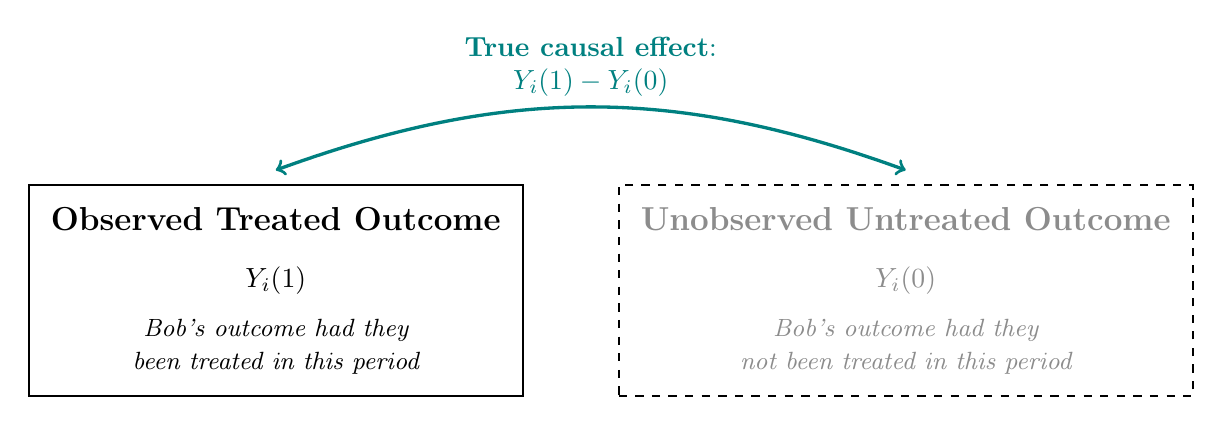
\begin{tikzpicture}[
    box/.style={draw, rectangle, minimum width=4cm, minimum height=2.5cm, align=center, inner sep=8pt},
    observed/.style={box, thick},
    unobserved/.style={box, dashed, thick, text=gray!90}
  ]

  % Potential outcomes boxes only
  \node[observed] (treated) at (-4,2) {
    \textbf{\large Observed Treated Outcome} \\[0.3cm]
    $Y_i(1)$ \\[0.2cm]
    {\small\itshape Bob's outcome had they} \\
    {\small\itshape been treated in this period}
  };

  \node[unobserved] (untreated) at (4,2) {
    \textbf{\large Unobserved Untreated Outcome} \\[0.3cm]
    $Y_i(0)$ \\[0.2cm]
    {\small\itshape Bob's outcome had they} \\
    {\small\itshape not been treated in this period}
  };

  % Arrow between potential outcomes
  \draw[<->, very thick, teal, bend left=20] 
    ([yshift=5pt]treated.north) to 
    node[midway, above, align=center] {
      \textbf{True causal effect}: \\ 
      $Y_i(1) - Y_i(0)$
    } 
    ([yshift=5pt]untreated.north);

  \end{tikzpicture}
}

\bigskip
For any individual, we can only observe \emph{one} of these potential outcomes, never both simultaneously
\end{frame}

\begin{frame}{Unit-level treatment effect}
  Define the \alert{unit-level treatment effect} to be $\tau_i = Y_i(1) - Y_i(0)$
  \begin{itemize}
    \item Measures the effect of $D_i$ from $0$ to $1$ on unit $i$
  \end{itemize}

  \bigskip
  Note this is for the \emph{same unit} at \emph{the same point in time}!
  
  \pause
  \begin{itemize}
    \item I am \emph{not} saying a neighborhood before and after the apartment is built (though this could be a way of trying to estimate a causal effect)
  \end{itemize}
\end{frame}

\begin{frame}{What do we oberve?}
  In our dataset, we observe average rent $Y_i$ and whether or not the aparmtent is built, $D_i$. How does this relate to potential outcomes?
  
  \bigskip
  The \alert{`switching equation'} relates potential outcomes to observed outcomes:
  $$
    Y_i = Y_i(1) D_i + Y_i(0) (1 - D_i)
  $$

  \pause
  \bigskip
  When $D_i = 1$, we have $Y_i = Y_i(1)$ and when $D_i = 0$ we have $Y_i = Y_i(0)$. That is, we observe \emph{one} of the two potential outcomes for each unit.
\end{frame}

\begin{frame}{Missing potential outcomes}
  \begin{columns}[T]
    \begin{column}{.4\textwidth}
      Here is the complete dataset
      \only<2>{
        \begin{itemize}
          \item However, we cannot actually observe the potential missing outcome!
          
          \item The goal is to use the \textbf{observed} observations to ``fill in'' the unobserved missing potential outcome
        \end{itemize}
      }
    \end{column}
    \begin{column}{.6\textwidth}\vspace*{-\bigskipamount}
      \begin{center}
        
        \begin{tabular}{@{}
          c@{\extracolsep{8pt}}cccc
        @{}} 
          \toprule
          $i$ & $D_i$ & $Y_i$ & $Y_i(1)$ & $Y_i(0)$ \\
          \midrule

          1 & 1 & \$1200 & \$1200 & \only<1>{\$1225}\only<2>{\color{purple} ?} \\
          2 & 0 & \$1000 & \only<1>{\$950}\only<2>{\color{purple} ?} & \$1000 \\
          3 & 1 & \$1150 & \$1150 & \only<1>{\$1150}\only<2>{\color{purple} ?}\\
          & & \vdots & & \\
          n & 0 & \$1100 & \only<1>{\$1090}\only<2>{\color{purple} ?} & \$1100 \\
      
          \bottomrule
        \end{tabular}
      \end{center}
    \end{column}
  \end{columns}
\end{frame}

\begin{frame}{Causal Estimands}
  \begin{columns}[T]
    \begin{column}{.4\textwidth}
      Recall our \alert{unit-level treatment effect} to be $\tau_i = Y_i(1) - Y_i(0)$
    \end{column}
    \begin{column}{.6\textwidth}\vspace*{-\bigskipamount}
      \begin{center}
        
        \begin{tabular}{@{}
          c@{\extracolsep{8pt}}ccccc
        @{}} 
          \toprule
          $i$ & $D_i$ & $Y_i$ & $Y_i(1)$ & $Y_i(0)$ & $\tau_i$ \\
          \midrule

          1 & 1 & \$1200 & \$1200 & \$1225 & -\$25 \\
          2 & 0 & \$1000 & \$950 & \$1000 & \$50 \\
          3 & 1 & \$1150 & \$1150 & \$1150 & \$0 \\
          & & \vdots & & \\
          n & 0 & \$1100 & \$1090 & \$1100 & -\$10 \\
      
          \bottomrule
        \end{tabular}
      \end{center}
    \end{column}
  \end{columns}
\end{frame}

\begin{frame}{Averaging unit-level treatment effects}
  Recall our \alert{unit-level treatment effect} to be $\tau_i = Y_i(1) - Y_i(0)$
  \begin{itemize}
    \item There is no reasonable way to estimate individual-level treatment effects (too much noise!)\pause, so we will aim to estimate \emph{averages} of them
  \end{itemize}

  \pause
  \bigskip
  The \alert{Average Treatment Effect} (ATE) is given by
  $$
    \tau_{\text{ATE}} = \expec{\tau_i} = \expec{Y_i(1) - Y_i(0)}
  $$
  \begin{itemize}
    \item This averages over every unit in your population (with equal weights), including those who never receive treatment
  \end{itemize}
\end{frame}

\begin{frame}{Causal Estimands}
  The ATE is useful if you are trying to understand the \textbf{average} effect of treatment on the entire population you are sampling from. 
  \begin{itemize}
    \item E.g. you are launching a pilot that you intend to scale up to the school level
    \pause
    \item Be careful; when scaling up a treatment, general equilibrium can change the impact of treatment! 
    \begin{itemize}
      \item One person getting resume tips is more useful then everyone getting resume tips
    \end{itemize}
  \end{itemize}

  \bigskip
  \pause
  This is less useful if you are trying to estimate the effect on a specific sub-population 
  \begin{itemize}
    \item Testing the effects of medicine on outcomes \emph{for the population with a disease}
  \end{itemize}
\end{frame}


\begin{frame}{Causal Estimands}
  There is the \alert{Average Treatment Effect on the Treated} (ATT) that averages over only units that receive treatment:
  $$
    \tau_{\text{ATT}} = \expec{\tau_i}{D_i = 1} = \expec{Y_i(1) - Y_i(0)}{D_i = 1}
  $$

  \bigskip
  \begin{itemize}
    \item In some cases, this will be the only estimate we can credibly identify
    
    \item If the treated population looks very different from the population as a whole, you face the risk of \alert{external validity} 
  \end{itemize}
\end{frame}

\begin{frame}{Causal Estimands}
  Likewise the \alert{Average Treatment Effect on the Control} (ATC) averages over only units that do not receive treatment:
  $$
    \tau_{\text{ATC}} = \expec{\tau_i}{D_i = 0} = \expec{Y_i(1) - Y_i(0)}{D_i = 0}
  $$
\end{frame}

\begin{frame}{Causal Estimands}
  All three estimands relate via the law of conditional expectations. Define $\pi = \prob{D_i = 1}$ be the probability of a unit being in treatment. 
  \begin{align*}
    \tau_{\text{ATE}} 
    &= \expec{\tau_i} = \expec{\expec{\tau_i}{D_i}} \\
    \pause
    &= \prob{D_i = 1} \expec{\tau_i}{D_i = 1} + \prob{D_i = 0} \expec{\tau_i}{D_i = 0} \\
    \pause
    &= \pi \tau_{\text{ATT}} + (1 - \pi) \tau_{\text{ATC}}  
  \end{align*}
\end{frame}

\begin{frame}{Conditional ATE}
  While an overall treatment effect is a useful summary measure, we often want to summarize treatment effects for \emph{groups of units with the same charactersitics}, e.g. gender, race, income, age, etc.
  
  \bigskip
  We define the \alert{Conditional Average Treatment Effect} (CATE) as:
  $$
    \tau_{\text{CATE}}(x) = \expec{\tau_i}{X_i = x} = \expec{Y_i(1) - Y_i(0)}{X_i = x}
  $$
  \begin{itemize}
    \item $X_i$ is some characteristic of the population
  \end{itemize}
\end{frame}

\begin{frame}{Conditional ATE versus ATE}
  There is a strong relationship between the CATE and the ATE/ATT:
  $$
    \tau_{\text{ATE}} = \expec{\tau_i} = \expec{\expec{\tau_i}{X_i}}
  $$
  \begin{itemize}
    \item The latter averages over CATE with weights proportional to the distribution of $X_i$ in the population
  \end{itemize}


  \pause
  \bigskip
  Likewise, we could average over the distribution of $X_i$ for the treated units
  $$
    \tau_{\text{ATT}} = \expec{\tau_i} = \expec{\tau_{\text{CATE}}(x)} = \expec{\expec{\tau_i}{X_i}}{D_i = 1}
  $$
\end{frame}

\begin{frame}{Problems with observational data}
  Our treatment effect parameter is given by 
  $$
    \tau_{\text{ATE}} = \expec{Y_{i}(1)} - \expec{Y_{i}(0)}
  $$
  
  \bigskip
  What if we replace expectations with sample averages for the treated and control groups?
  $$
    \hat{\tau}_{\text{DIM}} = \expec{Y_{i}}{D_i = 1} - \expec{Y_{i}}{D_i = 0}
  $$
  \begin{itemize}
    \item This is called the \alert{difference-in-means estimator}
  \end{itemize}
\end{frame}

% \begin{frame}{Difference-in-means estimator}
%   What does the difference-in-means estimator identify?
%   \begin{align*}
%     \hat{\tau}_{\text{DIM}} &= \expec{Y_{i}}{D_i = 1} - \expec{Y_{i}}{D_i = 0} \\
%     &= \expec{Y_{i}(1)}{D_i = 1} - \expec{Y_{i}(0)}{D_i = 0} \\
%     &= \expec{Y_{i}(1)}{D_i = 1} - \expec{Y_{i}(0)}{D_i = 0} \\
%     &\quad\quad - \expec{Y_{i}(1)} + \expec{Y_{i}(1)} - \expec{Y_{i}(0)} + \expec{Y_{i}(0)} \\[1em]
%     \pause
%     &= \tau_{\text{ATE}} + \left( \expec{Y_{i}(1)}{D_i = 1} - \expec{Y_{i}(1)} \right) - \left( \expec{Y_{i}(0)}{D_i = 0} - \expec{Y_{i}(0)} \right)
%   \end{align*}  
% 
%   So we identify the ATE plus two additional terms. Let's break them down
% \end{frame}
% 
% \begin{frame}{Difference-in-means estimator}
%   \vspace*{-2\bigskipamount}
%   $$
%     \hat{\tau}_{\text{DIM}} = 
%       \tau_{\text{ATE}} + {\color{orange} \left( \expec{Y_{i}(1)}{D_i = 1} - \expec{Y_{i}(1)} \right) - \left( \expec{Y_{i}(0)}{D_i = 0} - \expec{Y_{i}(0)} \right) }
%   $$
% 
%   The difference-in-means estimator will (generally) be not equal to the ATE if either of these terms are non-zero. 
%   
%   % TODO: Selection Bias
% \end{frame}

\begin{frame}{Difference-in-means estimator}
  What does the difference-in-means estimator identify? We can use the common ``add and subtract'' trick:
  \begin{align*}
    \hat{\tau}_{\text{DIM}} &= \expec{Y_{i}}{D_i = 1} - \expec{Y_{i}}{D_i = 0} \\
    &= \expec{Y_{i}(1)}{D_i = 1} - \expec{Y_{i}(0)}{D_i = 0} \\
    &= \expec{Y_{i}(1)}{D_i = 1} - \expec{Y_{i}(0)}{D_i = 0} - \expec{Y_{i}(0)}{D_i = 1} + \expec{Y_{i}(0)}{D_i = 1} \\[1em]
    \pause
    &= \tau_{\text{ATT}} + \left( \expec{Y_{i}(0)}{D_i = 1} - \expec{Y_{i}(0)}{D_i = 0} \right)
  \end{align*}  

  \bigskip
  The difference-in-means estimator equals the ATT plus an additional term.
\end{frame}

\begin{frame}{`Selection Bias'}
  We refer to the last term as {\color{orange} selection bias}
  $$
    \hat{\tau}_{\text{DIM}} = \tau_{\text{ATT}} + {\color{orange} \left( \expec{Y_{i}(0)}{D_i = 1} - \expec{Y_{i}(0)}{D_i = 0} \right) }
  $$

  \begin{itemize}
    \item If the treated group has a different mean untreated potential outcome than the control group, our estimator is biased.
  \end{itemize}

  \pause
  \bigskip
  For example, in our appartment example, the neighborhoods where apartments are built would have a higher \emph{counterfactual rent} (in the absence of a new apartment) than the untreated neighborhoods
  \begin{itemize}
    \item We would mistakingly claim this is due to new apartments being built!
  \end{itemize}
\end{frame}

\section{Randomized Experiments}

\begin{frame}{When is selection bias not present?}
  \vspace*{-\bigskipamount}
  $$
    \hat{\tau}_{\text{DIM}} = \tau_{\text{ATT}} + {\color{orange} \left( \expec{Y_{i}(0)}{D_i = 1} - \expec{Y_{i}(0)}{D_i = 0} \right) }
  $$

  \bigskip
  The leading example of when selection bias is not present is when $D_i$ is randomly assigned.
  
  \pause
  \bigskip
  When $D_i$ is randomly assigned, we have that the untreated potential outcome and treatment are independent: $(Y_i(0) \Perp D_i)$
  \begin{itemize}
    \item If $(Y_i(0) \Perp D_i)$, then $\expec{Y_{i}(0)}{D_i} = \expec{Y_{i}(0)}$ and selection bias is 0.

    \pause 
    \item Technically, we only need `mean-independence' which is the latter term; but in experiments, we have full independence.
  \end{itemize}
\end{frame}

\begin{frame}{Experiments and causal estimands}
  In fact, experiments help us estimate more than the ATT. Note that if we randomly assign treatment, then $(Y_i(1), Y_i(0)) \Perp D_i$. This means: 
  $$
    \expec{Y_i(1) - Y_i(0)}{D_i} = \expec{Y_i(1) - Y_i(0)}
  $$
  and hence $\text{ATE} = \text{ATT} = \text{ATC}$

  \begin{itemize}
    \item Since we randomly assign treatment, the treated group looks like the control group looks like the population as a whole.
  \end{itemize}
\end{frame}

\begin{frame}{`Balance Tables'}
  When running an experiment, it is common to collect information about the participants, call this information a vector $X_i$.

  \bigskip
  It is common to show that the randomization ``worked'' by showing that the distribution of $X_i$ is similar between treatment and control groups. 
  This is often done with a \alert{balance table} that shows means of $X_i$ by treatment status
\end{frame}



\begin{frame}{Quasi- and Natural Experiments}{Writing about Empirical Work}
  Often you will hear the terms `natural experiment' and `quasi-experimental design' in applied work
  \begin{itemize}
    \item There are appropriate and inappropriate usages of this term (in my opinion)
  \end{itemize}

  \bigskip
  If there are features of a research question in which we can think of $D_i$ as being randomly assigned (for a subgroup), then we can use the term `natural experiment' (in that it is naturally occuring)
  \begin{itemize}
    \item Angist (1990) uses the randomly assigned Vietnam-war draft
    \item Imbens, Rubin, and Sacerdote (2001) uses lottery winners which is randomly assigned among people who play the lottery
  \end{itemize}
\end{frame}

\begin{frame}{Observational Studies and ``Exogenous Variation''}{Writing about Empirical Work}
  In most contexts, you will not have a natural experiment. Instead, you will leverage variation in policies that we think is `exogenous' (e.g. the roll-out of policies or using details of the policy)

  \begin{itemize}
    \item In general, these papers require more work to do a good job at causally identifying effects
    
    \item E.g. states roll-out policies in response to their outcomes causing selection bias
  \end{itemize}

  \pause
  \bigskip
  All hope is not lost, though. The rest of the course will teach you strategies for estimating a causal effect
\end{frame}

\subsection{Estimation via Regression}

\begin{frame}{Regression estimates for experiments}
  The difference-in-means estimate is $\expec{Y_i}{D_i = 1} - \expec{Y_i}{D_i = 0}$
  \begin{itemize}
    \item We could, of course, estimate these means by hands (and you will be asked to do so on your assignment). 
  \end{itemize}

  However it is typically far simpler to run a regression because it will also give you (robust) standard errors. 
\end{frame}

\begin{frame}{Regression}
  The regression we will run is as follows:
  $$
    Y_i = \alpha + \tau D_i + \varepsilon_i
  $$
  Since $D_i$ is a dummy variable and $\alpha$ is the intercept, regression mechanics (which we'll talk about more in the next topic) tells us that 
  \begin{itemize}
    \item $\hat{\alpha} = \expechat{Y_i}{D_i = 0}$ and $\hat{\tau} = \expechat{Y_i}{D_i = 1} - \expechat{Y_i}{D_i = 0}$
  \end{itemize}

  \bigskip
  $\hat{\tau}$ is equal to our difference-in-means estimates! 
\end{frame}

\begin{frame}{Inference}
  Of course, we want to provide some measure of noise around our treatment effect estimates and be able to test the null that the ATE is equal to 0. 
  
  \bigskip
  Our difference-in-means estimator is given by
  $$
    \hat{\tau}_{\text{DIM}} = \frac{1}{n_1} \sum_{D_i = 1} Y_i - \frac{1}{n_0} \sum_{D_i = 0} Y_i
  $$

	\bigskip
  We will use the `weak null' (more on this in a second) that $\tau_{\text{ATT}} = 0$. 
	\begin{itemize}
		\item We will return in a few slides to discuss weak versus sharp null
	\end{itemize}
\end{frame}

\begin{frame}{Inference}
  The variance, under the null that $\tau = 0$, is given by
  $$
    \var{\hat{\tau}_{\text{DIM}}} = \expec{ \left( \frac{1}{n_1} \sum_{D_i = 1} Y_i - \frac{1}{n_0} \sum_{D_i = 0} Y_i \right)^2 }
  $$

  With a little algebra we can find
	\begin{align*}
		\var{\hat{\tau}_{\text{DIM}}} = \frac{1}{n_1} \var{Y_{i}(1)} + \frac{1}{n_0} \var{Y_{i}(0)}
	\end{align*}
	\begin{itemize}
		\item These variances can be estimated based on the variance within $D_i =
			1$ and $D_i = 0$ respectively. Randomization ensures consistency
	\end{itemize}
\end{frame}

\begin{frame}{Inference via Regression}
  Recall the regression we run is: 
	$$
    Y_i = \alpha + \tau D_i + \varepsilon_i
  $$

	Using robust standard errors, the variance estimate for $\hat{\tau}$ is approximately equal to the one on the previous slide. 
	\begin{itemize}
		\item Using HC2 standard errors give exact variance from above
	\end{itemize}
\end{frame}

% TODO: Randomization Inference



\subsection{LaLonde Dataset}

\begin{frame}{The start of the credibility revolution}
  LaLonde (1986) is a seminal work in the onset of the `credibility revolution' of causal inference to economics. The paper uses an experiment called the National Supported Work Demonstration (NSW) program

  \bigskip
  The program targeted randomly assigned a job training program to participants. The participants were drawn from `ex-drug addicts, ex-criminal offenders, and high-school dropouts'. 
\end{frame}

\begin{frame}{Experimental effects}
  Since treatment was randomly assigned, we can use the difference-in-means estimator to estimate the $\text{ATE} = \text{ATT} = \text{ATC}$
  \begin{itemize}
    \item Note that in the context of this experiment, the `population' we are thinking about is among the pool of participants
    \item It is not the ATE of the entire US population
  \end{itemize}
	
	\bigskip
	LaLonde found experimental evidence of about \$886 for male participants and \$851 for female participants
\end{frame}

\begin{frame}{LaLonde's test}
  LaLonde wanted to see what would happen if instead of using the experimental control group, he used observation data
	\begin{itemize}
		\item LaLonde brought in data from the Community Population Survey (CPS) and the Panel Study on Income Dynamics (PSID)  
	\end{itemize}

	\bigskip
	The `observational dataset', as he called it, consists of the treated units from the experiment and the control group from the survey data
	\pause
	\begin{itemize}
		\item Control group looks very different from the treated group (higher income, better job market attachments, higher education, etc.)
	\end{itemize}
\end{frame}

\begin{frame}{LaLonde's test}
	He used a simple regression:
	$$
		\text{wages}_i = \alpha + \tau D_i + X_i \beta + \varepsilon_i
	$$
	\begin{itemize}
		\item $X_i$ were a vector of controls (age, education, and race)
	\end{itemize}

	\pause \bigskip
	The estimates from this regression using the nonexperimental sample yielded significantly different results with many estimates coming out as negative!
\end{frame}

\begin{frame}{LaLonde's test}
	This was a very clever thing to do and led to many response articles trying to defend the then current methods
	\begin{itemize}
		\item Imbens and Xu (2024) present a really riviting account of the paper, responses, and modern solutions aimed to improve observational treatment effect estimates
	\end{itemize}

	\pause
	\bigskip
	Robert Lalonde, Orley Ashenfelter, David Card, and others in the Princeton Industrial Relations Section in the 1980s were drivers of the `credibility revolution'
\end{frame}




\section{A/B Testing}

\begin{frame}{A/B Testing}
  It is \emph{incredibly} common for firms to run many sets of experiments, which they call A/B testing
  \begin{itemize}
    \item Typically, it asks ``which performs better, version A or version B''
  \end{itemize}

	\bigskip
	For example, Youtubers will try to change their thumbnails randomly to different viewers and compare how often people click on the video 
\end{frame}

\begin{frame}{Difficulties with A/B Testing}
	Since this is effectively an experiment, understanding A/B testing should be simple; but it comes with some challenges:
  \begin{itemize}
		\item There can be many, many different `arms' in the experiment so you have many comparisons to make 

		\item As the experiment goes on, it is common to subset experimentation to the best-performing arms while dropping the worst performing (`adaptive bandit')
	\end{itemize}
\end{frame}

\begin{frame}{Multi-arm treatment effect estimates in A/B Testing}
  Our previous logic of randomization extends to an experiment where $D_i \in \{0, 1, \dots, K \}$ where $K + 1$ is the number of arms in the experiment.

	\bigskip
	Potential outcomes are given by $Y_i(D_i)$ and treatment effects are given by $\tau_i(d) = Y_{i}(d) - Y_{i}(0)$
	\pause
	\begin{itemize}
		\item If there is no natural `control group', then pick one randomly to normalize. Treatment effects are then `relative' to treatment 0
	\end{itemize}

	\bigskip
	Randomization ensures that $\left\{ Y_i(d) \right\}_{d=0}^K \Perp D_i$
\end{frame}

\begin{frame}{Multi-arm treatment effect estimates in A/B Testing}
	Treatment effects can be estimated using regression:
	$$
		Y_i = \alpha + \sum_{d = 1}^K \one{D_i = d} \tau^d + \varepsilon_i
	$$

	$\hat{\tau}^d$ are our treatment effect estimates
	\begin{itemize}
		\item Consistency comes from randomization (using similar math to the single treatment case)
	\end{itemize}
\end{frame}

\begin{frame}{Finding the `best' treatment}
	Say you want to chose treatment $d$ that has the largest treatment effect:
	$$
		\hat{d} = \argmax_{d \in \{1, \dots, K\}} \hat{\tau}(d)
	$$
	\begin{itemize}
		\item As the number of observations in each arm grows, this procedure asymptotically will select the best treatment arm
	\end{itemize}
\end{frame}

\begin{frame}{The Winner's Curse}
	For smaller sample sizes, this will face the `winner's curse' (Andrews, Kitagawa, and McCloskey (2024))
	\begin{itemize}
		\item The one with the highest effect is biased upwards by selecting on the error term
		\pause
		\item I've heard stories of tech companies running hundreds of arms with only a few observations per arm before picking a winner
	\end{itemize}

	\pause
	\bigskip
	The term comes from auction theory where $K$ bidders bid for the same product
	\begin{itemize}
		\item Even if each bidder can consistenly estimate the value, the highest bidder will have the highest valuation and overvalue the good
	\end{itemize}
\end{frame}

\begin{frame}{Finding the `best' treatment}
	Solutions to winner's curse:
	\begin{itemize}
		\item Use adaptive inference from Andrews, Kitagawa, and McCloskey (2024)
	\end{itemize}

	\bigskip
	What about doing more experimentation on the best arm's to disentangle?
\end{frame}

\begin{frame}{Multi-arm Bandit}
	A \alert{Multi-arm bandit} (sometimes called adaptive experiments) is a method of experimentation where the probability of being assigned to any arm changes over the course of the experiment
	\begin{itemize}
		\item It is costly to experiment, so lower the probability of treatment for arms that seem to not be good
	\end{itemize}

	\pause
	\bigskip
	This creates issues with inference since each observation depends on all previous observations (inducing dependence)
	\begin{itemize}
		\item Solutions exist, but we will skip the details in this class. See Hadad, Hirshberg, Zhan, Wager, and Athey (PNAS, 2021) for an example
	\end{itemize}
\end{frame}


% TODO: Covariates in Experiments

\end{document}
